\documentclass[a4paper,12pt,twoside]{article}
\usepackage[left=2cm, right=2cm, top=0.5cm, bottom=2.0cm, includeheadfoot]{geometry}
\usepackage{titlesec}
\usepackage{import}
\usepackage{amsmath, amssymb, amsfonts}
\usepackage{yhmath}
\usepackage{multirow}
\usepackage{graphicx}
\usepackage{mathspec}
\usepackage{parskip}
\usepackage{bm}
%\usepackage{xeCJK}
\usepackage{enumitem}
\usepackage{fancyhdr}
\usepackage{fancyvrb}
\usepackage{verbatim}
\usepackage{algorithm}
\usepackage{algorithmicx}
\usepackage{algpseudocode}
\usepackage{etoolbox}
\AtBeginEnvironment{quote}{\itshape}

\usepackage{tikz}
\usepackage{mathdots}
\usepackage{cancel}
\usepackage{color}
\usepackage{siunitx}
\usepackage{array}
\usepackage{multirow}
\usepackage{amssymb}
\usepackage{gensymb}
\usepackage{tabularx}
\usepackage{booktabs}
\usetikzlibrary{fadings}
\usetikzlibrary{patterns}

\titlespacing*{\subsection}{0pt}{0.5cm}{0.1cm}

\pagestyle{fancy}
\renewcommand{\headrulewidth}{0pt}

\lhead{}
\chead{\textsf{2019 China Multi-University Training Contest, Round 8} \\ \textsf{\small Aug. 14, 2019}}
\rhead{}
\lfoot{\textit{2019 China Multi-University Training 8, Problem \Alph{ProblemNo}: \ProblemName}}
\cfoot{}
\rfoot{\thepage}
%\setCJKmainfont[BoldFont=SimHei,ItalicFont=KaiTi]{SimSun}
\setmainfont[BoldFont=Arial Bold]{Times New Roman}
\setsansfont{Arial}
\setmonofont{Courier New}
%\setmathsfont(Latin){Times New Roman}

\setlist{nosep}
\newcommand{\ProblemName}{}
\newcommand{\ProblemID}{}
\newcounter{ProblemNo}
\newcounter{ExampleNo}

\newcommand{\exmpfilev}[1]{
    \begin{minipage}[t]{0.47\linewidth} \vspace{0cm} \verbatiminput{#1} \vspace{0.2cm} \end{minipage}
}
\newcommand{\exmpv}[1]{
    ~\\ [0.5cm]
    \addtocounter{ExampleNo}{1}
    \noindent
    \begin{tabular}{p{0.48\linewidth}p{0.48\linewidth}}
      \textbf{Sample Input \arabic{ExampleNo}} & \textbf{Sample Output \arabic{ExampleNo}} \\ \hline
    \multicolumn{1}{|l|}{\exmpfilev{#1.in}} & 
    \multicolumn{1}{l|} {\exmpfilev{#1.ans}} \\ \hline
    \end{tabular}
}
\newcommand{\exmph}[1]{
    ~\\ [0.5cm]
    \addtocounter{ExampleNo}{1}
    \noindent
    \begin{tabular}{p{0.98\linewidth}}
      \vspace{0cm}
      \textbf{Sample Input \arabic{ExampleNo}} \\ \hline
    \multicolumn{1}{|l|}{\exmpfilev{#1.in}} \\ \hline
      \vspace{0cm}
      \textbf{Sample Output \arabic{ExampleNo}} \\ \hline
    \multicolumn{1}{|l|} {\exmpfilev{#1.ans}} \\ \hline
    \end{tabular}
}
\newcommand{\problem}[1] {
    \renewcommand{\ProblemID}{#1}
    \documentclass[a4paper,12pt,twoside]{article}
\usepackage[left=2cm, right=2cm, top=0.5cm, bottom=2.0cm, includeheadfoot]{geometry}
\usepackage{titlesec}
\usepackage{import}
\usepackage{amsmath, amssymb, amsfonts}
\usepackage{yhmath}
\usepackage{multirow}
\usepackage{graphicx}
\usepackage{mathspec}
\usepackage{parskip}
\usepackage{bm}
%\usepackage{xeCJK}
\usepackage{enumitem}
\usepackage{fancyhdr}
\usepackage{fancyvrb}
\usepackage{verbatim}
\usepackage{algorithm}
\usepackage{algorithmicx}
\usepackage{algpseudocode}
\usepackage{etoolbox}
\AtBeginEnvironment{quote}{\itshape}

\usepackage{tikz}
\usepackage{mathdots}
\usepackage{cancel}
\usepackage{color}
\usepackage{siunitx}
\usepackage{array}
\usepackage{multirow}
\usepackage{amssymb}
\usepackage{gensymb}
\usepackage{tabularx}
\usepackage{booktabs}
\usetikzlibrary{fadings}
\usetikzlibrary{patterns}

\titlespacing*{\subsection}{0pt}{0.5cm}{0.1cm}

\pagestyle{fancy}
\renewcommand{\headrulewidth}{0pt}

\lhead{}
\chead{\textsf{2019 China Multi-University Training Contest, Round 8} \\ \textsf{\small Aug. 14, 2019}}
\rhead{}
\lfoot{\textit{2019 China Multi-University Training 8, Problem \Alph{ProblemNo}: \ProblemName}}
\cfoot{}
\rfoot{\thepage}
%\setCJKmainfont[BoldFont=SimHei,ItalicFont=KaiTi]{SimSun}
\setmainfont[BoldFont=Arial Bold]{Times New Roman}
\setsansfont{Arial}
\setmonofont{Courier New}
%\setmathsfont(Latin){Times New Roman}

\setlist{nosep}
\newcommand{\ProblemName}{}
\newcommand{\ProblemID}{}
\newcounter{ProblemNo}
\newcounter{ExampleNo}

\newcommand{\exmpfilev}[1]{
    \begin{minipage}[t]{0.47\linewidth} \vspace{0cm} \verbatiminput{#1} \vspace{0.2cm} \end{minipage}
}
\newcommand{\exmpv}[1]{
    ~\\ [0.5cm]
    \addtocounter{ExampleNo}{1}
    \noindent
    \begin{tabular}{p{0.48\linewidth}p{0.48\linewidth}}
      \textbf{Sample Input \arabic{ExampleNo}} & \textbf{Sample Output \arabic{ExampleNo}} \\ \hline
    \multicolumn{1}{|l|}{\exmpfilev{#1.in}} & 
    \multicolumn{1}{l|} {\exmpfilev{#1.ans}} \\ \hline
    \end{tabular}
}
\newcommand{\exmph}[1]{
    ~\\ [0.5cm]
    \addtocounter{ExampleNo}{1}
    \noindent
    \begin{tabular}{p{0.98\linewidth}}
      \vspace{0cm}
      \textbf{Sample Input \arabic{ExampleNo}} \\ \hline
    \multicolumn{1}{|l|}{\exmpfilev{#1.in}} \\ \hline
      \vspace{0cm}
      \textbf{Sample Output \arabic{ExampleNo}} \\ \hline
    \multicolumn{1}{|l|} {\exmpfilev{#1.ans}} \\ \hline
    \end{tabular}
}
\newcommand{\problem}[1] {
    \renewcommand{\ProblemID}{#1}
    \documentclass[a4paper,12pt,twoside]{article}
\usepackage[left=2cm, right=2cm, top=0.5cm, bottom=2.0cm, includeheadfoot]{geometry}
\usepackage{titlesec}
\usepackage{import}
\usepackage{amsmath, amssymb, amsfonts}
\usepackage{yhmath}
\usepackage{multirow}
\usepackage{graphicx}
\usepackage{mathspec}
\usepackage{parskip}
\usepackage{bm}
%\usepackage{xeCJK}
\usepackage{enumitem}
\usepackage{fancyhdr}
\usepackage{fancyvrb}
\usepackage{verbatim}
\usepackage{algorithm}
\usepackage{algorithmicx}
\usepackage{algpseudocode}
\usepackage{etoolbox}
\AtBeginEnvironment{quote}{\itshape}

\usepackage{tikz}
\usepackage{mathdots}
\usepackage{cancel}
\usepackage{color}
\usepackage{siunitx}
\usepackage{array}
\usepackage{multirow}
\usepackage{amssymb}
\usepackage{gensymb}
\usepackage{tabularx}
\usepackage{booktabs}
\usetikzlibrary{fadings}
\usetikzlibrary{patterns}

\titlespacing*{\subsection}{0pt}{0.5cm}{0.1cm}

\pagestyle{fancy}
\renewcommand{\headrulewidth}{0pt}

\lhead{}
\chead{\textsf{2019 China Multi-University Training Contest, Round 8} \\ \textsf{\small Aug. 14, 2019}}
\rhead{}
\lfoot{\textit{2019 China Multi-University Training 8, Problem \Alph{ProblemNo}: \ProblemName}}
\cfoot{}
\rfoot{\thepage}
%\setCJKmainfont[BoldFont=SimHei,ItalicFont=KaiTi]{SimSun}
\setmainfont[BoldFont=Arial Bold]{Times New Roman}
\setsansfont{Arial}
\setmonofont{Courier New}
%\setmathsfont(Latin){Times New Roman}

\setlist{nosep}
\newcommand{\ProblemName}{}
\newcommand{\ProblemID}{}
\newcounter{ProblemNo}
\newcounter{ExampleNo}

\newcommand{\exmpfilev}[1]{
    \begin{minipage}[t]{0.47\linewidth} \vspace{0cm} \verbatiminput{#1} \vspace{0.2cm} \end{minipage}
}
\newcommand{\exmpv}[1]{
    ~\\ [0.5cm]
    \addtocounter{ExampleNo}{1}
    \noindent
    \begin{tabular}{p{0.48\linewidth}p{0.48\linewidth}}
      \textbf{Sample Input \arabic{ExampleNo}} & \textbf{Sample Output \arabic{ExampleNo}} \\ \hline
    \multicolumn{1}{|l|}{\exmpfilev{#1.in}} & 
    \multicolumn{1}{l|} {\exmpfilev{#1.ans}} \\ \hline
    \end{tabular}
}
\newcommand{\exmph}[1]{
    ~\\ [0.5cm]
    \addtocounter{ExampleNo}{1}
    \noindent
    \begin{tabular}{p{0.98\linewidth}}
      \vspace{0cm}
      \textbf{Sample Input \arabic{ExampleNo}} \\ \hline
    \multicolumn{1}{|l|}{\exmpfilev{#1.in}} \\ \hline
      \vspace{0cm}
      \textbf{Sample Output \arabic{ExampleNo}} \\ \hline
    \multicolumn{1}{|l|} {\exmpfilev{#1.ans}} \\ \hline
    \end{tabular}
}
\newcommand{\problem}[1] {
    \renewcommand{\ProblemID}{#1}
    \documentclass[a4paper,12pt,twoside]{article}
\usepackage[left=2cm, right=2cm, top=0.5cm, bottom=2.0cm, includeheadfoot]{geometry}
\usepackage{titlesec}
\usepackage{import}
\usepackage{amsmath, amssymb, amsfonts}
\usepackage{yhmath}
\usepackage{multirow}
\usepackage{graphicx}
\usepackage{mathspec}
\usepackage{parskip}
\usepackage{bm}
%\usepackage{xeCJK}
\usepackage{enumitem}
\usepackage{fancyhdr}
\usepackage{fancyvrb}
\usepackage{verbatim}
\usepackage{algorithm}
\usepackage{algorithmicx}
\usepackage{algpseudocode}
\usepackage{etoolbox}
\AtBeginEnvironment{quote}{\itshape}

\usepackage{tikz}
\usepackage{mathdots}
\usepackage{cancel}
\usepackage{color}
\usepackage{siunitx}
\usepackage{array}
\usepackage{multirow}
\usepackage{amssymb}
\usepackage{gensymb}
\usepackage{tabularx}
\usepackage{booktabs}
\usetikzlibrary{fadings}
\usetikzlibrary{patterns}

\titlespacing*{\subsection}{0pt}{0.5cm}{0.1cm}

\pagestyle{fancy}
\renewcommand{\headrulewidth}{0pt}

\lhead{}
\chead{\textsf{2019 China Multi-University Training Contest, Round 8} \\ \textsf{\small Aug. 14, 2019}}
\rhead{}
\lfoot{\textit{2019 China Multi-University Training 8, Problem \Alph{ProblemNo}: \ProblemName}}
\cfoot{}
\rfoot{\thepage}
%\setCJKmainfont[BoldFont=SimHei,ItalicFont=KaiTi]{SimSun}
\setmainfont[BoldFont=Arial Bold]{Times New Roman}
\setsansfont{Arial}
\setmonofont{Courier New}
%\setmathsfont(Latin){Times New Roman}

\setlist{nosep}
\newcommand{\ProblemName}{}
\newcommand{\ProblemID}{}
\newcounter{ProblemNo}
\newcounter{ExampleNo}

\newcommand{\exmpfilev}[1]{
    \begin{minipage}[t]{0.47\linewidth} \vspace{0cm} \verbatiminput{#1} \vspace{0.2cm} \end{minipage}
}
\newcommand{\exmpv}[1]{
    ~\\ [0.5cm]
    \addtocounter{ExampleNo}{1}
    \noindent
    \begin{tabular}{p{0.48\linewidth}p{0.48\linewidth}}
      \textbf{Sample Input \arabic{ExampleNo}} & \textbf{Sample Output \arabic{ExampleNo}} \\ \hline
    \multicolumn{1}{|l|}{\exmpfilev{#1.in}} & 
    \multicolumn{1}{l|} {\exmpfilev{#1.ans}} \\ \hline
    \end{tabular}
}
\newcommand{\exmph}[1]{
    ~\\ [0.5cm]
    \addtocounter{ExampleNo}{1}
    \noindent
    \begin{tabular}{p{0.98\linewidth}}
      \vspace{0cm}
      \textbf{Sample Input \arabic{ExampleNo}} \\ \hline
    \multicolumn{1}{|l|}{\exmpfilev{#1.in}} \\ \hline
      \vspace{0cm}
      \textbf{Sample Output \arabic{ExampleNo}} \\ \hline
    \multicolumn{1}{|l|} {\exmpfilev{#1.ans}} \\ \hline
    \end{tabular}
}
\newcommand{\problem}[1] {
    \renewcommand{\ProblemID}{#1}
    \input{contest/\ProblemID/statement/stat.tex}
}

\newenvironment{Problem}[2]{
    \addtocounter{ProblemNo}{1}
    \renewcommand{\ProblemName}{#1}
    \setcounter{ExampleNo}{0}
    \begin{center}
    \textsf{
        \huge{Problem \Alph{ProblemNo}} \\[0.1cm]
        \LARGE{\ProblemName} \\[0.2cm]
        \large{Time limit: #2 \ifnum#2=1 second \else seconds \fi} \\ [0.6cm]
    }
    \end{center}
}{
    \clearpage
}
\raggedbottom

\begin{document}
\vspace*{-0.5cm}
%\input{stammering.tex}
\input{cube.tex}
\input{girl.tex}
\input{number.tex}
\input{hunting.tex}
\input{string.tex}
\input{travel.tex}
\input{ds.tex}
\input{maze.tex}
\input{landlord.tex}
\input{ccpc.tex}
\input{milk.tex}
\end{document}

}

\newenvironment{Problem}[2]{
    \addtocounter{ProblemNo}{1}
    \renewcommand{\ProblemName}{#1}
    \setcounter{ExampleNo}{0}
    \begin{center}
    \textsf{
        \huge{Problem \Alph{ProblemNo}} \\[0.1cm]
        \LARGE{\ProblemName} \\[0.2cm]
        \large{Time limit: #2 \ifnum#2=1 second \else seconds \fi} \\ [0.6cm]
    }
    \end{center}
}{
    \clearpage
}
\raggedbottom

\begin{document}
\vspace*{-0.5cm}
%\input{stammering.tex}
\begin{Problem}{Acesrc and Cube Hypernet}{2}

Given a 3-dimensional cube, if we cut some edges, the surface of the cube can be unfolded into 2-dimensional space. Such flat shape is called a \textit{cube net}. There are 11 essentially different cube nets, listed below.

\begin{figure}[htb]
\centering
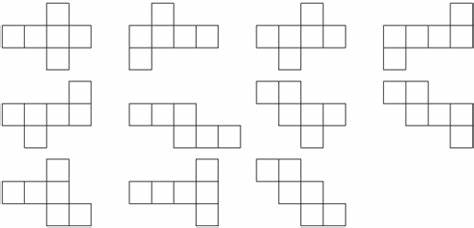
\includegraphics[width=12cm]{nets.jpg}
\caption{The 11 essentially different cube nets.}
\end{figure}

In this problem, we consider a generalization of the cube net, called \textit{cube hypernet}. For each face of a cube, we divide it into $k \times k$ small square cells. If we cut some edges of these small cells, the surface of the cube can be unfolded into 2-dimensional space, then the resulting flat shape is a cube hypernet. Clearly, cube nets are just a special type of cube hypernets where $k = 1$. The following picture illustrates a cube hypernet and explains how it is formed.

\begin{figure}[htb]
\centering

\tikzset{every picture/.style={line width=0.75pt}} %set default line width to 0.75pt        

\begin{tikzpicture}[x=0.75pt,y=0.75pt,yscale=-1,xscale=1]
%uncomment if require: \path (0,300); %set diagram left start at 0, and has height of 300

%Shape: Cube [id:dp5713421173433544] 
\draw   (92,119.87) -- (124.2,87.67) -- (199.43,87.67) -- (199.43,162.8) -- (167.23,195) -- (92,195) -- cycle ; \draw   (199.43,87.67) -- (167.23,119.87) -- (92,119.87) ; \draw   (167.23,119.87) -- (167.23,195) ;
%Straight Lines [id:da42563945957545957] 
\draw [color={rgb, 255:red, 208; green, 2; blue, 27 }  ,draw opacity=1 ][line width=3]    (92,119.87) -- (92,195) ;


%Straight Lines [id:da11360839227996866] 
\draw [color={rgb, 255:red, 208; green, 2; blue, 27 }  ,draw opacity=1 ][line width=3]    (92,119.87) -- (167.23,119.87) ;


%Straight Lines [id:da5837990090607357] 
\draw [color={rgb, 255:red, 208; green, 2; blue, 27 }  ,draw opacity=1 ][line width=3]  [dash pattern={on 7.88pt off 4.5pt}]  (124.2,87.67) -- (124.22,163.49) ;


%Straight Lines [id:da3949397955529803] 
\draw [color={rgb, 255:red, 208; green, 2; blue, 27 }  ,draw opacity=1 ][line width=3]    (125.08,86.84) -- (199.43,87.67) ;


%Straight Lines [id:da4851398910346689] 
\draw [color={rgb, 255:red, 208; green, 2; blue, 27 }  ,draw opacity=1 ][line width=3]    (167.23,119.87) -- (167.23,195) ;


%Straight Lines [id:da7311203923035952] 
\draw [color={rgb, 255:red, 208; green, 2; blue, 27 }  ,draw opacity=1 ][line width=3]    (199.43,87.67) -- (198.57,164.32) ;


%Straight Lines [id:da7022479459425415] 
\draw  [dash pattern={on 4.5pt off 4.5pt}]  (124.22,163.49) -- (199.43,162.8) ;


%Straight Lines [id:da7189806870957662] 
\draw  [dash pattern={on 4.5pt off 4.5pt}]  (124.22,163.49) -- (92,195) ;


%Straight Lines [id:da9178045604326999] 
\draw [color={rgb, 255:red, 0; green, 0; blue, 0 }  ,draw opacity=1 ] [dash pattern={on 0.84pt off 2.51pt}]  (145.93,104.17) -- (182.43,104.67) ;


%Straight Lines [id:da04301172838480838] 
\draw [color={rgb, 255:red, 0; green, 0; blue, 0 }  ,draw opacity=1 ] [dash pattern={on 0.84pt off 2.51pt}]  (92,157.43) -- (167.23,157.43) ;


%Straight Lines [id:da9145997008953277] 
\draw [color={rgb, 255:red, 0; green, 0; blue, 0 }  ,draw opacity=1 ] [dash pattern={on 0.84pt off 2.51pt}]  (129.61,120.12) -- (129.61,194.75) ;


%Straight Lines [id:da9400584505703131] 
\draw  [dash pattern={on 0.84pt off 2.51pt}]  (109.43,103.67) -- (109.43,176.67) ;


%Straight Lines [id:da4339187022384017] 
\draw  [dash pattern={on 0.84pt off 2.51pt}]  (92,157.43) -- (123.43,126.01) ;


%Straight Lines [id:da12326295357742123] 
\draw  [dash pattern={on 0.84pt off 2.51pt}]  (109.43,176.67) -- (183.43,176.67) ;


%Straight Lines [id:da859413357855844] 
\draw  [dash pattern={on 0.84pt off 2.51pt}]  (129.61,194.75) -- (161.82,163.15) ;


%Straight Lines [id:da22416829329673393] 
\draw  [dash pattern={on 0.84pt off 2.51pt}]  (162.25,87.25) -- (161.82,163.15) ;


%Straight Lines [id:da5602089262552088] 
\draw  [dash pattern={on 0.84pt off 2.51pt}]  (124.21,125.58) -- (199,125.99) ;


%Straight Lines [id:da9523299030375125] 
\draw  [dash pattern={on 0.84pt off 2.51pt}]  (167.23,157.43) -- (199,125.99) ;


%Straight Lines [id:da5451371565037118] 
\draw  [dash pattern={on 0.84pt off 2.51pt}]  (182.43,104.67) -- (183.43,176.67) ;


%Shape: Square [id:dp7591135470696151] 
\draw   (390,65) -- (414.33,65) -- (414.33,89.33) -- (390,89.33) -- cycle ;
%Shape: Square [id:dp917157522376586] 
\draw   (390,89.33) -- (414.33,89.33) -- (414.33,113.67) -- (390,113.67) -- cycle ;
%Shape: Square [id:dp6066190461876488] 
\draw   (414.33,65) -- (438.67,65) -- (438.67,89.33) -- (414.33,89.33) -- cycle ;
%Shape: Square [id:dp23412140295087092] 
\draw   (414.33,89.33) -- (438.67,89.33) -- (438.67,113.67) -- (414.33,113.67) -- cycle ;
%Shape: Square [id:dp39521998722950746] 
\draw   (390,113.67) -- (414.33,113.67) -- (414.33,138) -- (390,138) -- cycle ;
%Shape: Square [id:dp7597028280692992] 
\draw   (390,138) -- (414.33,138) -- (414.33,162.33) -- (390,162.33) -- cycle ;
%Shape: Square [id:dp9032016100512299] 
\draw   (414.33,113.67) -- (438.67,113.67) -- (438.67,138) -- (414.33,138) -- cycle ;
%Shape: Square [id:dp9862136660298677] 
\draw   (414.33,138) -- (438.67,138) -- (438.67,162.33) -- (414.33,162.33) -- cycle ;
%Shape: Square [id:dp2105696458351256] 
\draw   (390,162.33) -- (414.33,162.33) -- (414.33,186.67) -- (390,186.67) -- cycle ;
%Shape: Square [id:dp38203525928531445] 
\draw   (414.33,162.33) -- (438.67,162.33) -- (438.67,186.67) -- (414.33,186.67) -- cycle ;
%Shape: Square [id:dp07452681855437948] 
\draw   (390,186.67) -- (414.33,186.67) -- (414.33,211) -- (390,211) -- cycle ;
%Shape: Square [id:dp46685422276231514] 
\draw   (414.33,186.67) -- (438.67,186.67) -- (438.67,211) -- (414.33,211) -- cycle ;
%Shape: Square [id:dp1815129932944446] 
\draw   (438.67,113.67) -- (463,113.67) -- (463,138) -- (438.67,138) -- cycle ;
%Shape: Square [id:dp8928307047272608] 
\draw   (438.67,138) -- (463,138) -- (463,162.33) -- (438.67,162.33) -- cycle ;
%Shape: Square [id:dp3917633232801916] 
\draw   (463,113.67) -- (487.34,113.67) -- (487.34,138) -- (463,138) -- cycle ;
%Shape: Square [id:dp4091908537319717] 
\draw   (463,138) -- (487.34,138) -- (487.34,162.33) -- (463,162.33) -- cycle ;
%Shape: Square [id:dp3525235222171257] 
\draw   (365.67,113.67) -- (390,113.67) -- (390,138) -- (365.67,138) -- cycle ;
%Shape: Square [id:dp5339668640142305] 
\draw   (365.67,138) -- (390,138) -- (390,162.33) -- (365.67,162.33) -- cycle ;
%Shape: Square [id:dp8907339502163012] 
\draw   (341.33,113.67) -- (365.67,113.67) -- (365.67,138) -- (341.33,138) -- cycle ;
%Shape: Square [id:dp4554401476147847] 
\draw   (341.33,138) -- (365.67,138) -- (365.67,162.33) -- (341.33,162.33) -- cycle ;
%Shape: Square [id:dp633196329874429] 
\draw   (317,113.67) -- (341.33,113.67) -- (341.33,138) -- (317,138) -- cycle ;
%Shape: Square [id:dp062935463038297] 
\draw   (511.67,138) -- (536,138) -- (536,162.33) -- (511.67,162.33) -- cycle ;
%Shape: Square [id:dp8856843680936886] 
\draw   (487.34,113.67) -- (511.67,113.67) -- (511.67,138) -- (487.34,138) -- cycle ;
%Shape: Square [id:dp514905839618633] 
\draw   (487.34,138) -- (511.67,138) -- (511.67,162.33) -- (487.34,162.33) -- cycle ;
%Straight Lines [id:da9682499505773039] 
\draw [color={rgb, 255:red, 208; green, 2; blue, 27 }  ,draw opacity=1 ][line width=3]    (145.93,104.17) -- (162.25,87.25) ;


%Straight Lines [id:da17272908888168392] 
\draw [color={rgb, 255:red, 208; green, 2; blue, 27 }  ,draw opacity=1 ][line width=3.75]    (109.43,103.67) -- (145.93,104.17) ;


%Straight Lines [id:da7081830858409768] 
\draw [color={rgb, 255:red, 208; green, 2; blue, 27 }  ,draw opacity=1 ][line width=3.75]    (109.43,103.67) -- (92,119.87) ;


%Straight Lines [id:da379429243876815] 
\draw  [dash pattern={on 0.84pt off 2.51pt}]  (145.93,104.17) -- (129.61,120.12) ;


\end{tikzpicture}
\caption{A cube hypernet.}
\end{figure}

Identifying cube nets is a relatively easy job, however, this might not be true for cube hypernets. Here comes the challenge. Given a flat shape composed of small squares, determine whether it is a cube hypernet.

\subsection*{Input}

The first line of the input is a single integer $T$ $(1 \leq T \leq 30)$, denoting the number of test cases. 

For each test case, the first line contains two integers $h, w$ $(1 \leq h, w \leq 100)$, denoting the height and width of the input region. For the remaining $h$ lines, each containing $w$ characters, either \texttt{'\#'} or \texttt{'.'}. The character \texttt{'\#'} means that the square is part of the shape, while the character \texttt{'.'} means that the square is not part of the shape.

It is guaranteed that the input shape is nonempty and connected in four directions, and there is no hole inside the shape, not even a hole 8-connected to the outside. Also, the sum of $h \times w$ over all test cases does not exceed 35000.

\subsection*{Output}

For each test case, output \texttt{yes} in a line if the input shape is cube hypernet, and \texttt{no} otherwise.

\exmpv{cube}

\end{Problem}

\begin{Problem}{Acesrc and Girlfriend}{12}

Acesrc and his girlfriend are famous sweet lovers at Nanjing University second to none. They often wander along the streets near Xinjiekou, and taste takoyaki.

Xinjiekou is the central business district of Nanjing, consisting of $n$ crossroads and $m$ streets connecting some pairs of these crossroads. By every street there is a takoyaki bar, and Acesrc has a preference value for each of these bars. The streets are bidirectional.

Acesrc and his girlfriend choose a pair of crossroads as the starting point and the ending point; moreover, they choose a route between these two crossroads, and they walk along the streets in the route. Every crossroad appears in the route at most once. Once they encounter a takoyaki bar they will buy a serve of takoyaki from this bar. However, they can keep at most two serves of takoyaki. If, after buying a serve of takoyaki they have more than two serves, they will discard one serve with minimum preference value.

After reaching the ending point they begin to enjoy the takoyaki. Acesrc always eats the serve with lower preference value; however, if they only bought one serve, poor Acesrc will have nothing to eat. The clever Acesrc wants to know the minimum possible preference value of the serve he eats, given the starting point and the ending point of their route. Can you tell him the value?

\subsection*{Input}

The first line of input consists of a single integer $T$ $(1 \leq T \leq 100)$, the number of test cases. 

For each test case, the first line consists of three integers $n, m, q$ $(1 \leq n, q \leq 10^5, 1 \leq m \leq 2 \times 10^5)$, denoting the number of crossroads, streets in Xinjiekou, and the number of queries, respectively. Each of the next $m$ lines contains three integers $x, y, w$ $(1 \leq x, y \leq n, x \neq y, 1 \leq w \leq 10^9)$, denoting a street connecting the $x$th and the $y$th crossroads, with a takoyaki bar of preference value $w$ near the street. It is possible that multiple streets connect the same pair of crossroads. Each of the last $q$ lines are two integers $u, v$ $(1 \leq u, v \leq n, u \neq v)$, specifying a query that the starting point and ending point are the $u$th and the $v$th crossroads, respectively.

It is guaranteed that the sum of $n$ and the sum of $q$ over all test cases do not exceed $2.5 \times 10^5$, and the sum of $m$ does not exceed $5 \times 10^5$.

\subsection*{Output}

For each query of each test case, print the answer in one line. If Acesrc might have nothing to eat, print 0; if there is no path between the given starting and ending point, print -1.

\exmpv{girl}

\end{Problem}

\begin{Problem}{Acesrc and Good Numbers}{1}

Acesrc is a famous mathematician at Nanjing University second to none. Playing with interesting numbers is his favorite. Today, he finds a manuscript when cleaning his room, which reads

\begin{quote}
... Let $f(d, n)$ denote the number of occurrences of digit $d$ in decimal representations of integers $1, 2, 3, \cdots, n$. The function has some fantastic properties ...

... Obviously, there exist some nonnegative integers $k$, such that $f(d, k) = k$, and I decide to call them $d$-good numbers ...

... I have found all $d$-good numbers not exceeding $10^{1000}$, but the paper is too small to write all these numbers ...
\end{quote}

Acesrc quickly recollects all $d$-good numbers he found, and he tells Zou a question about $d$-good numbers: what is the maximum $d$-good number no greater than $x$? However, Zou is not good at mathematics, so he wants you to help him solve this problem.

\subsection*{Input}

The first line of input consists of a single integer $q$ $(1 \leq q \leq 1500)$, denoting the number of test cases. Each test case is a single line with two integers $d$ $(1 \leq d \leq 9)$ and $x$ $(0 \leq x \leq 10^{18})$.

\subsection*{Output}

For each test case, print the answer as a single integer in one line. Note that $0$ is trivially a $d$-good number for arbitrary $d$.

\exmpv{number}

\end{Problem}

\begin{Problem}{Acesrc and Hunting}{2}

Acesrc is a famous hunter at Nanjing University second to none. Recently, he set $n \times m$ traps in Yangshan Park, a park near Nanjing University Xianlin Campus, arranged in $n$ rows and $m$ columns. The rows are numbered $1$ through $n$ from bottom to up, and the columns are numbered $1$ through $m$ from left to right. The distance between two adjacent traps, both horizontally and vertically, is 1 meter.

Today, Acesrc happily finds that every trap he set has captured an animal. He decides to collect these hunted animals to make roast meat for his friends. However, collecting these animals normally is too boring, so he decides to find a route following the rules below:
\begin{itemize}
\item Acesrc can choose any trap to start; every time he collects the animal in the trap, and moves to some unvisited trap until all animals captured are collected;
\item The Euclidean distance he moves from one trap to the next trap should be between 1 meter and 3 meters exclusive; that is, the distance should be strictly greater than 1 meter and strictly less than 3 meters.
\end{itemize}

Acesrc has quickly collected all animals. Roo wonders how Acesrc collected these animals, but Acesrc buttons up his lip. Can you give a possible route to collect all the animals?

\subsection*{Input}

The first line of input consists of a single integer $T$ $(1 \leq T \leq 240)$, the number of test cases. Each test case is a single line of two integers $n, m$ $(1 \leq n, m \leq 100)$, denoting the size of the trap matrix.

\subsection*{Output}

For each test case, if it is impossible to find any valid route, print \texttt{NO} in a single line; otherwise, print \texttt{YES} in one line, followed by $n \times m$ lines describing the route, each of these lines containing two integers $x, y$ $(1 \leq x \leq n, 1 \leq y \leq m)$, denoting the position of a trap visited. If multiple solutions exist, print any.

\exmpv{hunting}

\end{Problem}

\begin{Problem}{Acesrc and String Theory}{7}

Acesrc is a famous string theorist at Nanjing University second to none. He insists on the principle that we should say an important thing $k$ times. He believes that every string that can be obtained by concatenating $k$ copies of some nonempty string is splendid. So, he always teaches newcomers, ``String theory problems are important! String theory problems are important! ... String theory problems are important!"

Today, he wants to examine whether the newcomers remember his instruction. He presents a string consisting of lower case letters and asks them the number of splendid substrings of the presented string. No one can solve this problem, and they will be scolded for hours. Can you help them solve this problem?

Note that equal splendid substrings occurred in different positions should be counted multiple times.

\subsection*{Input}

The first line of input consists of a single integer $T$ $(1 \leq T \leq 10)$, denoting the number of test cases. Each test case starts with a single line of an integer $k$ $(1 \leq k \leq 20)$. The second line of a test case is a string $S$ consisting of lower case letters only, the length of which is between $1$ and $3 \times 10^5$ inclusive. The sum of the lengths of all strings does not exceed $10^6$.

\subsection*{Output}

For each test case, print the answer as a single integer in a single line.

\exmpv{string}

\end{Problem}

\begin{Problem}{Acesrc and Travel}{2}

Acesrc is a famous tourist at Nanjing University second to none. During this summer holiday, he, along with Zhang and Liu, is going to travel to Hong Kong. There are $n$ spots in Hong Kong, and $n - 1$ bidirectional sightseeing bus routes connecting these spots. They decide to visit some spots by taking the buses.

However, Zhang and Liu have different preferences for these spots. They respectively set a satisfactory value for each spot. If they visit the $i$th spot, Zhang will obtain satisfactory value $a_i$, and Liu will obtain $b_i$. Starting with Zhang, they alternately decide the next spot to visit for the sake of fairness. There must be a bus route between the current spot and the next spot to visit. Moreover, they would never like to visit a spot twice. If anyone can't find such a next spot to visit, they have no choice but to end this travel.

Zhang and Liu are both super smart competitive programmers. Either want to maximize the difference between his total satisfactory value and the other's. Now Acesrc wonders, if they both choose optimally, what is the difference of total satisfactory values of Zhang and Liu?

\subsection*{Input}

The first line of input consists of a single integer $T$ $(1 \leq T \leq 30)$, denoting the number of test cases.

For each test case, the first line contains a single integer $n$ $(1 \leq n \leq 10^5)$, denoting the number of spots. Each of the next two lines contains $n$ integers, $a_1, a_2, \cdots, a_n$ and $b_1, b_2, \cdots, b_n$ $(0 \leq a_i, b_i \leq 10^9)$, denoting the 
satisfactory value of Zhang and Liu for every spot, respectively. Each of the last $n - 1$ lines contains two integers $x, y$ $(1 \leq x, y \leq n, x \neq y)$, denoting a bus route between the $x$th spot and the $y$th spot. It is reachable from any spot to any other spot through these bus routes.

It is guaranteed that the sum of $n$ does not exceed $5.01 \times 10^5$.

\subsection*{Output}

For each test case, print a single integer in one line, the difference of total satisfactory values if they both choose optimally.

\exmpv{travel}

\end{Problem}

\begin{Problem}{Andy and Data Structure}{15}

Andy is a famous data structure expert at Nanjing University second to none. One day he throws a plain dry data structure problem to his friends, but none of them can solve. How about you?

Given a tree rooted at node 1. Each node has a weight which is 0 initially. Define the distance between two nodes as the number of edges in the unique simple path between the two nodes. You need to perform these two types of operations:
\begin{itemize}
\item Type 1: given $a, x, y, z$, add $z$ to the weights of all $a$'s descendants (including $a$ itself) whose distances to $a$ are $x$ modulo $y$;
\item Type 2: given $a$, return the weight associated with node $a$.
\end{itemize}

\subsection*{Input}

The first line of the input is a single integer $T$ $(1 \leq T \leq 3)$, the number of test cases.

Each test cases starts with two integers $n, m$ $(1 \leq n, m \leq 300000)$, denoting that there are $n$ nodes (numbered $1$ through $n$) in the tree and you need to perform $m$ operations. The next line contains $n-1$ integers, $f_1, f_2, \cdots, f_{n-1}$ $(1 \leq f_i \leq i)$, specifying the edges of the trees; the $i$th integer denotes the parent of node $i+1$. The next $m$ lines describe the operations. Each line is either \texttt{1 a x y z} $(1 \leq a \leq n, 1 \leq x \leq n, 0 \leq y < x, 0 \leq z \leq 500)$, denoting an operation of type 1, or \texttt{2 a} $(1 \leq a \leq n)$, denoting an operation of type 2.

\subsection*{Output}

For each operation of type 2 in each test case, print the answer in one line.

\exmpv{ds}

\end{Problem}

\begin{Problem}{Andy and Maze}{15}

Andy is a famous explorer at Nanjing University second to none. One day he was trapped in a maze. The maze consisted of several rooms, and there was a precious gem in each room. There were also some bidirectional roads connecting some pairs of these rooms. It took some time to travel along the road in either direction.

Andy was in a room, but he didn't know which room he was in. Suddenly, he heard a low voice, saying that, ``if you want to get out of the maze, you must collect $k$ gems." Andy wanted to know, what was the minimum possible time to get out of the maze, or it was impossible at all? Note that he couldn't visit the same room more than once.

\subsection*{Input}

The first line of input consists of a single integer $T$ $(1 \leq T \leq 30)$, denoting the number of test cases. Each test case starts with a line of three integers $n, m, k$ $(2 \leq n \leq 10^4, 1 \leq m \leq 10^4, 2 \leq k \leq 6)$, denoting the number of rooms and the number of roads in the maze, and the number of gems he needed collect, respectively. The next $m$ lines, each containing three intergers $u, v, t$ $(1 \leq u, v \leq n, u \neq v, 1 \leq t \leq 10^8)$, specifying a road connecting the $u$th and the $v$th rooms, which takes $t$ minutes to travel in either direction. No two roads connect the same pair of rooms.
There are at most 5 test cases with $\max\{n, m\} > 100$.

\subsection*{Output}

For each test case, print the minimum possible time in minute to get out of the maze in one line. If it was impossible to get out of the maze, print \texttt{impossible} instead.

\exmpv{maze}

\end{Problem}

\begin{Problem}{Calabash and Landlord}{1}

Calabash is the servant of a landlord. The landlord owns a piece of land, which can be regarded as an infinite 2D plane.

One day the landlord set up two orthogonal rectangular-shaped fences on his land. He asked Calabash a simple problem: how many nonempty connected components is my land divided into by these two fences, both finite and infinite? Calabash couldn't answer this simple question. Please help him! 

Recall that a connected component is a maximal set of points not occupied by the fences, and every two points in the set are reachable without crossing the fence.

\subsection*{Input}

The first line of input consists of a single integer $T$ $(1 \leq T \leq 10000)$, the number of test cases. 

Each test case contains two lines, specifying the two rectangles. Each line contains four integers $x_1, y_1, x_2, y_2$ $(0 \leq x_1, y_1, x_2, y_2 \leq 10^9, x_1 < x_2, y_1 < y_2)$, where $(x_1, y_1), (x_2, y_2)$ are the Cartesian coordinates of two opposite vertices of the rectangular fence. The edges of the rectangles are parallel to the coordinate axes. The edges of the two rectangles may intersect, overlap, or even coincide.

\subsection*{Output}

For each test case, print the answer as an integer in one line.

\exmpv{landlord}

\end{Problem}

\begin{Problem}{Quailty and CCPC}{2}

Considering the overall difficulty of other problems, we invite Quailty to propose an easy problem for this contest.

Quailty accidentally won both gold medal and silver medal in 2017 CCPC final. The reason is explained as follows. According to the official rule, the number of gold medals was 10\% of the number of participating teams, rounded to the nearest integer. This is ambiguous when the fractional part of the result is exactly $0.5$. There were 115 participating teams, and the rank of Quailty's team was 12. The organizer originally decided to round down the number, so there were only 11 gold medals, and Quailty's team could only win the silver medal. Many people defended him against the organizer, saying that his team deserved the gold medal. Later, the organizer changed to round up the number, and Quailty's team finally won a gold medal.

Now, give you the scoreboard of a contest and the proportion of gold medal teams, could you determine whether there exists a team, such that they would win a gold medal were the number of gold medals rounded up when the fractional part is exactly $0.5$, and silver medal if rounded down?

A team ranks before another if they solved more problems or both teams solved an equal number of problems but they had less penalty time.

\textit{(Disclaimer: the background is fictitious and the problem is prepared by Nanjing University ICPC Training Team, not Quailty.)}

\subsection*{Input}

The first line of input consists of a single integer $T$ $(1 \leq T \leq 120)$, denoting the number of test cases.

Each test case starts with a line of two integers $n$ $(1 \leq n \leq 10^5)$, denoting the number of participating teams, and $d$ $(0 \leq d \leq 9)$, denoting that the proportion of gold medal teams is $10d\%$. For the next $n$ lines, each containing a string $s$ and two integers $p, t$ $(0 \leq p, t \leq 10^9)$, denoting the name of the team, the number of problems solved and the penalty time of the team, respectively. The name of the each team contains at least 1 and at most 10 latin letters. The names are case sensitive. No two teams have the same name. No two teams have the same penalty time. The sum of $n$ over all test cases does not exceed $10^6$.

\subsection*{Output}

For each test case, print the team name if there exists such team, or print \texttt{Quailty is very great} otherwise. It can be proved that there is at most one such team.

\exmpv{ccpc}

\end{Problem}

\begin{Problem}{Roundgod and Milk Tea}{5}

Roundgod is a famous milk tea lover at Nanjing University second to none. This year, he plans to conduct a milk tea festival. There will be $n$ classes participating in this festival, where the $i$th class has $a_i$ students and will make $b_i$ cups of milk tea.

Roundgod wants more students to savor milk tea, so he stipulates that every student can taste at most one cup of milk tea. Moreover, a student can't drink a cup of milk tea made by his class. The problem is, what is the maximum number of students who can drink milk tea?

\subsection*{Input}

The first line of input consists of a single integer $T$ $(1 \leq T \leq 25)$, denoting the number of test cases.

Each test case starts with a line of a single integer $n$ $(1 \leq n \leq 10^6)$, the number of classes. For the next $n$ lines, each containing two integers $a, b$ $(0 \leq a, b \leq 10^9)$, denoting the number of students of the class and the number of cups of milk tea made by this class, respectively.

It is guaranteed that the sum of $n$ over all test cases does not exceed $6 \times 10^6$.

\subsection*{Output}

For each test case, print the answer as a single integer in one line.

\exmpv{milk}

\end{Problem}

\end{document}

}

\newenvironment{Problem}[2]{
    \addtocounter{ProblemNo}{1}
    \renewcommand{\ProblemName}{#1}
    \setcounter{ExampleNo}{0}
    \begin{center}
    \textsf{
        \huge{Problem \Alph{ProblemNo}} \\[0.1cm]
        \LARGE{\ProblemName} \\[0.2cm]
        \large{Time limit: #2 \ifnum#2=1 second \else seconds \fi} \\ [0.6cm]
    }
    \end{center}
}{
    \clearpage
}
\raggedbottom

\begin{document}
\vspace*{-0.5cm}
%\input{stammering.tex}
\begin{Problem}{Acesrc and Cube Hypernet}{2}

Given a 3-dimensional cube, if we cut some edges, the surface of the cube can be unfolded into 2-dimensional space. Such flat shape is called a \textit{cube net}. There are 11 essentially different cube nets, listed below.

\begin{figure}[htb]
\centering
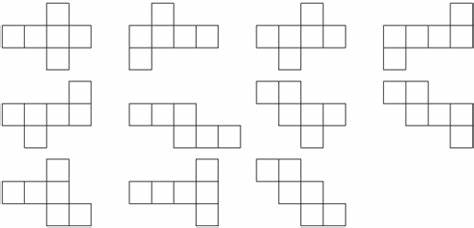
\includegraphics[width=12cm]{nets.jpg}
\caption{The 11 essentially different cube nets.}
\end{figure}

In this problem, we consider a generalization of the cube net, called \textit{cube hypernet}. For each face of a cube, we divide it into $k \times k$ small square cells. If we cut some edges of these small cells, the surface of the cube can be unfolded into 2-dimensional space, then the resulting flat shape is a cube hypernet. Clearly, cube nets are just a special type of cube hypernets where $k = 1$. The following picture illustrates a cube hypernet and explains how it is formed.

\begin{figure}[htb]
\centering

\tikzset{every picture/.style={line width=0.75pt}} %set default line width to 0.75pt        

\begin{tikzpicture}[x=0.75pt,y=0.75pt,yscale=-1,xscale=1]
%uncomment if require: \path (0,300); %set diagram left start at 0, and has height of 300

%Shape: Cube [id:dp5713421173433544] 
\draw   (92,119.87) -- (124.2,87.67) -- (199.43,87.67) -- (199.43,162.8) -- (167.23,195) -- (92,195) -- cycle ; \draw   (199.43,87.67) -- (167.23,119.87) -- (92,119.87) ; \draw   (167.23,119.87) -- (167.23,195) ;
%Straight Lines [id:da42563945957545957] 
\draw [color={rgb, 255:red, 208; green, 2; blue, 27 }  ,draw opacity=1 ][line width=3]    (92,119.87) -- (92,195) ;


%Straight Lines [id:da11360839227996866] 
\draw [color={rgb, 255:red, 208; green, 2; blue, 27 }  ,draw opacity=1 ][line width=3]    (92,119.87) -- (167.23,119.87) ;


%Straight Lines [id:da5837990090607357] 
\draw [color={rgb, 255:red, 208; green, 2; blue, 27 }  ,draw opacity=1 ][line width=3]  [dash pattern={on 7.88pt off 4.5pt}]  (124.2,87.67) -- (124.22,163.49) ;


%Straight Lines [id:da3949397955529803] 
\draw [color={rgb, 255:red, 208; green, 2; blue, 27 }  ,draw opacity=1 ][line width=3]    (125.08,86.84) -- (199.43,87.67) ;


%Straight Lines [id:da4851398910346689] 
\draw [color={rgb, 255:red, 208; green, 2; blue, 27 }  ,draw opacity=1 ][line width=3]    (167.23,119.87) -- (167.23,195) ;


%Straight Lines [id:da7311203923035952] 
\draw [color={rgb, 255:red, 208; green, 2; blue, 27 }  ,draw opacity=1 ][line width=3]    (199.43,87.67) -- (198.57,164.32) ;


%Straight Lines [id:da7022479459425415] 
\draw  [dash pattern={on 4.5pt off 4.5pt}]  (124.22,163.49) -- (199.43,162.8) ;


%Straight Lines [id:da7189806870957662] 
\draw  [dash pattern={on 4.5pt off 4.5pt}]  (124.22,163.49) -- (92,195) ;


%Straight Lines [id:da9178045604326999] 
\draw [color={rgb, 255:red, 0; green, 0; blue, 0 }  ,draw opacity=1 ] [dash pattern={on 0.84pt off 2.51pt}]  (145.93,104.17) -- (182.43,104.67) ;


%Straight Lines [id:da04301172838480838] 
\draw [color={rgb, 255:red, 0; green, 0; blue, 0 }  ,draw opacity=1 ] [dash pattern={on 0.84pt off 2.51pt}]  (92,157.43) -- (167.23,157.43) ;


%Straight Lines [id:da9145997008953277] 
\draw [color={rgb, 255:red, 0; green, 0; blue, 0 }  ,draw opacity=1 ] [dash pattern={on 0.84pt off 2.51pt}]  (129.61,120.12) -- (129.61,194.75) ;


%Straight Lines [id:da9400584505703131] 
\draw  [dash pattern={on 0.84pt off 2.51pt}]  (109.43,103.67) -- (109.43,176.67) ;


%Straight Lines [id:da4339187022384017] 
\draw  [dash pattern={on 0.84pt off 2.51pt}]  (92,157.43) -- (123.43,126.01) ;


%Straight Lines [id:da12326295357742123] 
\draw  [dash pattern={on 0.84pt off 2.51pt}]  (109.43,176.67) -- (183.43,176.67) ;


%Straight Lines [id:da859413357855844] 
\draw  [dash pattern={on 0.84pt off 2.51pt}]  (129.61,194.75) -- (161.82,163.15) ;


%Straight Lines [id:da22416829329673393] 
\draw  [dash pattern={on 0.84pt off 2.51pt}]  (162.25,87.25) -- (161.82,163.15) ;


%Straight Lines [id:da5602089262552088] 
\draw  [dash pattern={on 0.84pt off 2.51pt}]  (124.21,125.58) -- (199,125.99) ;


%Straight Lines [id:da9523299030375125] 
\draw  [dash pattern={on 0.84pt off 2.51pt}]  (167.23,157.43) -- (199,125.99) ;


%Straight Lines [id:da5451371565037118] 
\draw  [dash pattern={on 0.84pt off 2.51pt}]  (182.43,104.67) -- (183.43,176.67) ;


%Shape: Square [id:dp7591135470696151] 
\draw   (390,65) -- (414.33,65) -- (414.33,89.33) -- (390,89.33) -- cycle ;
%Shape: Square [id:dp917157522376586] 
\draw   (390,89.33) -- (414.33,89.33) -- (414.33,113.67) -- (390,113.67) -- cycle ;
%Shape: Square [id:dp6066190461876488] 
\draw   (414.33,65) -- (438.67,65) -- (438.67,89.33) -- (414.33,89.33) -- cycle ;
%Shape: Square [id:dp23412140295087092] 
\draw   (414.33,89.33) -- (438.67,89.33) -- (438.67,113.67) -- (414.33,113.67) -- cycle ;
%Shape: Square [id:dp39521998722950746] 
\draw   (390,113.67) -- (414.33,113.67) -- (414.33,138) -- (390,138) -- cycle ;
%Shape: Square [id:dp7597028280692992] 
\draw   (390,138) -- (414.33,138) -- (414.33,162.33) -- (390,162.33) -- cycle ;
%Shape: Square [id:dp9032016100512299] 
\draw   (414.33,113.67) -- (438.67,113.67) -- (438.67,138) -- (414.33,138) -- cycle ;
%Shape: Square [id:dp9862136660298677] 
\draw   (414.33,138) -- (438.67,138) -- (438.67,162.33) -- (414.33,162.33) -- cycle ;
%Shape: Square [id:dp2105696458351256] 
\draw   (390,162.33) -- (414.33,162.33) -- (414.33,186.67) -- (390,186.67) -- cycle ;
%Shape: Square [id:dp38203525928531445] 
\draw   (414.33,162.33) -- (438.67,162.33) -- (438.67,186.67) -- (414.33,186.67) -- cycle ;
%Shape: Square [id:dp07452681855437948] 
\draw   (390,186.67) -- (414.33,186.67) -- (414.33,211) -- (390,211) -- cycle ;
%Shape: Square [id:dp46685422276231514] 
\draw   (414.33,186.67) -- (438.67,186.67) -- (438.67,211) -- (414.33,211) -- cycle ;
%Shape: Square [id:dp1815129932944446] 
\draw   (438.67,113.67) -- (463,113.67) -- (463,138) -- (438.67,138) -- cycle ;
%Shape: Square [id:dp8928307047272608] 
\draw   (438.67,138) -- (463,138) -- (463,162.33) -- (438.67,162.33) -- cycle ;
%Shape: Square [id:dp3917633232801916] 
\draw   (463,113.67) -- (487.34,113.67) -- (487.34,138) -- (463,138) -- cycle ;
%Shape: Square [id:dp4091908537319717] 
\draw   (463,138) -- (487.34,138) -- (487.34,162.33) -- (463,162.33) -- cycle ;
%Shape: Square [id:dp3525235222171257] 
\draw   (365.67,113.67) -- (390,113.67) -- (390,138) -- (365.67,138) -- cycle ;
%Shape: Square [id:dp5339668640142305] 
\draw   (365.67,138) -- (390,138) -- (390,162.33) -- (365.67,162.33) -- cycle ;
%Shape: Square [id:dp8907339502163012] 
\draw   (341.33,113.67) -- (365.67,113.67) -- (365.67,138) -- (341.33,138) -- cycle ;
%Shape: Square [id:dp4554401476147847] 
\draw   (341.33,138) -- (365.67,138) -- (365.67,162.33) -- (341.33,162.33) -- cycle ;
%Shape: Square [id:dp633196329874429] 
\draw   (317,113.67) -- (341.33,113.67) -- (341.33,138) -- (317,138) -- cycle ;
%Shape: Square [id:dp062935463038297] 
\draw   (511.67,138) -- (536,138) -- (536,162.33) -- (511.67,162.33) -- cycle ;
%Shape: Square [id:dp8856843680936886] 
\draw   (487.34,113.67) -- (511.67,113.67) -- (511.67,138) -- (487.34,138) -- cycle ;
%Shape: Square [id:dp514905839618633] 
\draw   (487.34,138) -- (511.67,138) -- (511.67,162.33) -- (487.34,162.33) -- cycle ;
%Straight Lines [id:da9682499505773039] 
\draw [color={rgb, 255:red, 208; green, 2; blue, 27 }  ,draw opacity=1 ][line width=3]    (145.93,104.17) -- (162.25,87.25) ;


%Straight Lines [id:da17272908888168392] 
\draw [color={rgb, 255:red, 208; green, 2; blue, 27 }  ,draw opacity=1 ][line width=3.75]    (109.43,103.67) -- (145.93,104.17) ;


%Straight Lines [id:da7081830858409768] 
\draw [color={rgb, 255:red, 208; green, 2; blue, 27 }  ,draw opacity=1 ][line width=3.75]    (109.43,103.67) -- (92,119.87) ;


%Straight Lines [id:da379429243876815] 
\draw  [dash pattern={on 0.84pt off 2.51pt}]  (145.93,104.17) -- (129.61,120.12) ;


\end{tikzpicture}
\caption{A cube hypernet.}
\end{figure}

Identifying cube nets is a relatively easy job, however, this might not be true for cube hypernets. Here comes the challenge. Given a flat shape composed of small squares, determine whether it is a cube hypernet.

\subsection*{Input}

The first line of the input is a single integer $T$ $(1 \leq T \leq 30)$, denoting the number of test cases. 

For each test case, the first line contains two integers $h, w$ $(1 \leq h, w \leq 100)$, denoting the height and width of the input region. For the remaining $h$ lines, each containing $w$ characters, either \texttt{'\#'} or \texttt{'.'}. The character \texttt{'\#'} means that the square is part of the shape, while the character \texttt{'.'} means that the square is not part of the shape.

It is guaranteed that the input shape is nonempty and connected in four directions, and there is no hole inside the shape, not even a hole 8-connected to the outside. Also, the sum of $h \times w$ over all test cases does not exceed 35000.

\subsection*{Output}

For each test case, output \texttt{yes} in a line if the input shape is cube hypernet, and \texttt{no} otherwise.

\exmpv{cube}

\end{Problem}

\begin{Problem}{Acesrc and Girlfriend}{12}

Acesrc and his girlfriend are famous sweet lovers at Nanjing University second to none. They often wander along the streets near Xinjiekou, and taste takoyaki.

Xinjiekou is the central business district of Nanjing, consisting of $n$ crossroads and $m$ streets connecting some pairs of these crossroads. By every street there is a takoyaki bar, and Acesrc has a preference value for each of these bars. The streets are bidirectional.

Acesrc and his girlfriend choose a pair of crossroads as the starting point and the ending point; moreover, they choose a route between these two crossroads, and they walk along the streets in the route. Every crossroad appears in the route at most once. Once they encounter a takoyaki bar they will buy a serve of takoyaki from this bar. However, they can keep at most two serves of takoyaki. If, after buying a serve of takoyaki they have more than two serves, they will discard one serve with minimum preference value.

After reaching the ending point they begin to enjoy the takoyaki. Acesrc always eats the serve with lower preference value; however, if they only bought one serve, poor Acesrc will have nothing to eat. The clever Acesrc wants to know the minimum possible preference value of the serve he eats, given the starting point and the ending point of their route. Can you tell him the value?

\subsection*{Input}

The first line of input consists of a single integer $T$ $(1 \leq T \leq 100)$, the number of test cases. 

For each test case, the first line consists of three integers $n, m, q$ $(1 \leq n, q \leq 10^5, 1 \leq m \leq 2 \times 10^5)$, denoting the number of crossroads, streets in Xinjiekou, and the number of queries, respectively. Each of the next $m$ lines contains three integers $x, y, w$ $(1 \leq x, y \leq n, x \neq y, 1 \leq w \leq 10^9)$, denoting a street connecting the $x$th and the $y$th crossroads, with a takoyaki bar of preference value $w$ near the street. It is possible that multiple streets connect the same pair of crossroads. Each of the last $q$ lines are two integers $u, v$ $(1 \leq u, v \leq n, u \neq v)$, specifying a query that the starting point and ending point are the $u$th and the $v$th crossroads, respectively.

It is guaranteed that the sum of $n$ and the sum of $q$ over all test cases do not exceed $2.5 \times 10^5$, and the sum of $m$ does not exceed $5 \times 10^5$.

\subsection*{Output}

For each query of each test case, print the answer in one line. If Acesrc might have nothing to eat, print 0; if there is no path between the given starting and ending point, print -1.

\exmpv{girl}

\end{Problem}

\begin{Problem}{Acesrc and Good Numbers}{1}

Acesrc is a famous mathematician at Nanjing University second to none. Playing with interesting numbers is his favorite. Today, he finds a manuscript when cleaning his room, which reads

\begin{quote}
... Let $f(d, n)$ denote the number of occurrences of digit $d$ in decimal representations of integers $1, 2, 3, \cdots, n$. The function has some fantastic properties ...

... Obviously, there exist some nonnegative integers $k$, such that $f(d, k) = k$, and I decide to call them $d$-good numbers ...

... I have found all $d$-good numbers not exceeding $10^{1000}$, but the paper is too small to write all these numbers ...
\end{quote}

Acesrc quickly recollects all $d$-good numbers he found, and he tells Zou a question about $d$-good numbers: what is the maximum $d$-good number no greater than $x$? However, Zou is not good at mathematics, so he wants you to help him solve this problem.

\subsection*{Input}

The first line of input consists of a single integer $q$ $(1 \leq q \leq 1500)$, denoting the number of test cases. Each test case is a single line with two integers $d$ $(1 \leq d \leq 9)$ and $x$ $(0 \leq x \leq 10^{18})$.

\subsection*{Output}

For each test case, print the answer as a single integer in one line. Note that $0$ is trivially a $d$-good number for arbitrary $d$.

\exmpv{number}

\end{Problem}

\begin{Problem}{Acesrc and Hunting}{2}

Acesrc is a famous hunter at Nanjing University second to none. Recently, he set $n \times m$ traps in Yangshan Park, a park near Nanjing University Xianlin Campus, arranged in $n$ rows and $m$ columns. The rows are numbered $1$ through $n$ from bottom to up, and the columns are numbered $1$ through $m$ from left to right. The distance between two adjacent traps, both horizontally and vertically, is 1 meter.

Today, Acesrc happily finds that every trap he set has captured an animal. He decides to collect these hunted animals to make roast meat for his friends. However, collecting these animals normally is too boring, so he decides to find a route following the rules below:
\begin{itemize}
\item Acesrc can choose any trap to start; every time he collects the animal in the trap, and moves to some unvisited trap until all animals captured are collected;
\item The Euclidean distance he moves from one trap to the next trap should be between 1 meter and 3 meters exclusive; that is, the distance should be strictly greater than 1 meter and strictly less than 3 meters.
\end{itemize}

Acesrc has quickly collected all animals. Roo wonders how Acesrc collected these animals, but Acesrc buttons up his lip. Can you give a possible route to collect all the animals?

\subsection*{Input}

The first line of input consists of a single integer $T$ $(1 \leq T \leq 240)$, the number of test cases. Each test case is a single line of two integers $n, m$ $(1 \leq n, m \leq 100)$, denoting the size of the trap matrix.

\subsection*{Output}

For each test case, if it is impossible to find any valid route, print \texttt{NO} in a single line; otherwise, print \texttt{YES} in one line, followed by $n \times m$ lines describing the route, each of these lines containing two integers $x, y$ $(1 \leq x \leq n, 1 \leq y \leq m)$, denoting the position of a trap visited. If multiple solutions exist, print any.

\exmpv{hunting}

\end{Problem}

\begin{Problem}{Acesrc and String Theory}{7}

Acesrc is a famous string theorist at Nanjing University second to none. He insists on the principle that we should say an important thing $k$ times. He believes that every string that can be obtained by concatenating $k$ copies of some nonempty string is splendid. So, he always teaches newcomers, ``String theory problems are important! String theory problems are important! ... String theory problems are important!"

Today, he wants to examine whether the newcomers remember his instruction. He presents a string consisting of lower case letters and asks them the number of splendid substrings of the presented string. No one can solve this problem, and they will be scolded for hours. Can you help them solve this problem?

Note that equal splendid substrings occurred in different positions should be counted multiple times.

\subsection*{Input}

The first line of input consists of a single integer $T$ $(1 \leq T \leq 10)$, denoting the number of test cases. Each test case starts with a single line of an integer $k$ $(1 \leq k \leq 20)$. The second line of a test case is a string $S$ consisting of lower case letters only, the length of which is between $1$ and $3 \times 10^5$ inclusive. The sum of the lengths of all strings does not exceed $10^6$.

\subsection*{Output}

For each test case, print the answer as a single integer in a single line.

\exmpv{string}

\end{Problem}

\begin{Problem}{Acesrc and Travel}{2}

Acesrc is a famous tourist at Nanjing University second to none. During this summer holiday, he, along with Zhang and Liu, is going to travel to Hong Kong. There are $n$ spots in Hong Kong, and $n - 1$ bidirectional sightseeing bus routes connecting these spots. They decide to visit some spots by taking the buses.

However, Zhang and Liu have different preferences for these spots. They respectively set a satisfactory value for each spot. If they visit the $i$th spot, Zhang will obtain satisfactory value $a_i$, and Liu will obtain $b_i$. Starting with Zhang, they alternately decide the next spot to visit for the sake of fairness. There must be a bus route between the current spot and the next spot to visit. Moreover, they would never like to visit a spot twice. If anyone can't find such a next spot to visit, they have no choice but to end this travel.

Zhang and Liu are both super smart competitive programmers. Either want to maximize the difference between his total satisfactory value and the other's. Now Acesrc wonders, if they both choose optimally, what is the difference of total satisfactory values of Zhang and Liu?

\subsection*{Input}

The first line of input consists of a single integer $T$ $(1 \leq T \leq 30)$, denoting the number of test cases.

For each test case, the first line contains a single integer $n$ $(1 \leq n \leq 10^5)$, denoting the number of spots. Each of the next two lines contains $n$ integers, $a_1, a_2, \cdots, a_n$ and $b_1, b_2, \cdots, b_n$ $(0 \leq a_i, b_i \leq 10^9)$, denoting the 
satisfactory value of Zhang and Liu for every spot, respectively. Each of the last $n - 1$ lines contains two integers $x, y$ $(1 \leq x, y \leq n, x \neq y)$, denoting a bus route between the $x$th spot and the $y$th spot. It is reachable from any spot to any other spot through these bus routes.

It is guaranteed that the sum of $n$ does not exceed $5.01 \times 10^5$.

\subsection*{Output}

For each test case, print a single integer in one line, the difference of total satisfactory values if they both choose optimally.

\exmpv{travel}

\end{Problem}

\begin{Problem}{Andy and Data Structure}{15}

Andy is a famous data structure expert at Nanjing University second to none. One day he throws a plain dry data structure problem to his friends, but none of them can solve. How about you?

Given a tree rooted at node 1. Each node has a weight which is 0 initially. Define the distance between two nodes as the number of edges in the unique simple path between the two nodes. You need to perform these two types of operations:
\begin{itemize}
\item Type 1: given $a, x, y, z$, add $z$ to the weights of all $a$'s descendants (including $a$ itself) whose distances to $a$ are $x$ modulo $y$;
\item Type 2: given $a$, return the weight associated with node $a$.
\end{itemize}

\subsection*{Input}

The first line of the input is a single integer $T$ $(1 \leq T \leq 3)$, the number of test cases.

Each test cases starts with two integers $n, m$ $(1 \leq n, m \leq 300000)$, denoting that there are $n$ nodes (numbered $1$ through $n$) in the tree and you need to perform $m$ operations. The next line contains $n-1$ integers, $f_1, f_2, \cdots, f_{n-1}$ $(1 \leq f_i \leq i)$, specifying the edges of the trees; the $i$th integer denotes the parent of node $i+1$. The next $m$ lines describe the operations. Each line is either \texttt{1 a x y z} $(1 \leq a \leq n, 1 \leq x \leq n, 0 \leq y < x, 0 \leq z \leq 500)$, denoting an operation of type 1, or \texttt{2 a} $(1 \leq a \leq n)$, denoting an operation of type 2.

\subsection*{Output}

For each operation of type 2 in each test case, print the answer in one line.

\exmpv{ds}

\end{Problem}

\begin{Problem}{Andy and Maze}{15}

Andy is a famous explorer at Nanjing University second to none. One day he was trapped in a maze. The maze consisted of several rooms, and there was a precious gem in each room. There were also some bidirectional roads connecting some pairs of these rooms. It took some time to travel along the road in either direction.

Andy was in a room, but he didn't know which room he was in. Suddenly, he heard a low voice, saying that, ``if you want to get out of the maze, you must collect $k$ gems." Andy wanted to know, what was the minimum possible time to get out of the maze, or it was impossible at all? Note that he couldn't visit the same room more than once.

\subsection*{Input}

The first line of input consists of a single integer $T$ $(1 \leq T \leq 30)$, denoting the number of test cases. Each test case starts with a line of three integers $n, m, k$ $(2 \leq n \leq 10^4, 1 \leq m \leq 10^4, 2 \leq k \leq 6)$, denoting the number of rooms and the number of roads in the maze, and the number of gems he needed collect, respectively. The next $m$ lines, each containing three intergers $u, v, t$ $(1 \leq u, v \leq n, u \neq v, 1 \leq t \leq 10^8)$, specifying a road connecting the $u$th and the $v$th rooms, which takes $t$ minutes to travel in either direction. No two roads connect the same pair of rooms.
There are at most 5 test cases with $\max\{n, m\} > 100$.

\subsection*{Output}

For each test case, print the minimum possible time in minute to get out of the maze in one line. If it was impossible to get out of the maze, print \texttt{impossible} instead.

\exmpv{maze}

\end{Problem}

\begin{Problem}{Calabash and Landlord}{1}

Calabash is the servant of a landlord. The landlord owns a piece of land, which can be regarded as an infinite 2D plane.

One day the landlord set up two orthogonal rectangular-shaped fences on his land. He asked Calabash a simple problem: how many nonempty connected components is my land divided into by these two fences, both finite and infinite? Calabash couldn't answer this simple question. Please help him! 

Recall that a connected component is a maximal set of points not occupied by the fences, and every two points in the set are reachable without crossing the fence.

\subsection*{Input}

The first line of input consists of a single integer $T$ $(1 \leq T \leq 10000)$, the number of test cases. 

Each test case contains two lines, specifying the two rectangles. Each line contains four integers $x_1, y_1, x_2, y_2$ $(0 \leq x_1, y_1, x_2, y_2 \leq 10^9, x_1 < x_2, y_1 < y_2)$, where $(x_1, y_1), (x_2, y_2)$ are the Cartesian coordinates of two opposite vertices of the rectangular fence. The edges of the rectangles are parallel to the coordinate axes. The edges of the two rectangles may intersect, overlap, or even coincide.

\subsection*{Output}

For each test case, print the answer as an integer in one line.

\exmpv{landlord}

\end{Problem}

\begin{Problem}{Quailty and CCPC}{2}

Considering the overall difficulty of other problems, we invite Quailty to propose an easy problem for this contest.

Quailty accidentally won both gold medal and silver medal in 2017 CCPC final. The reason is explained as follows. According to the official rule, the number of gold medals was 10\% of the number of participating teams, rounded to the nearest integer. This is ambiguous when the fractional part of the result is exactly $0.5$. There were 115 participating teams, and the rank of Quailty's team was 12. The organizer originally decided to round down the number, so there were only 11 gold medals, and Quailty's team could only win the silver medal. Many people defended him against the organizer, saying that his team deserved the gold medal. Later, the organizer changed to round up the number, and Quailty's team finally won a gold medal.

Now, give you the scoreboard of a contest and the proportion of gold medal teams, could you determine whether there exists a team, such that they would win a gold medal were the number of gold medals rounded up when the fractional part is exactly $0.5$, and silver medal if rounded down?

A team ranks before another if they solved more problems or both teams solved an equal number of problems but they had less penalty time.

\textit{(Disclaimer: the background is fictitious and the problem is prepared by Nanjing University ICPC Training Team, not Quailty.)}

\subsection*{Input}

The first line of input consists of a single integer $T$ $(1 \leq T \leq 120)$, denoting the number of test cases.

Each test case starts with a line of two integers $n$ $(1 \leq n \leq 10^5)$, denoting the number of participating teams, and $d$ $(0 \leq d \leq 9)$, denoting that the proportion of gold medal teams is $10d\%$. For the next $n$ lines, each containing a string $s$ and two integers $p, t$ $(0 \leq p, t \leq 10^9)$, denoting the name of the team, the number of problems solved and the penalty time of the team, respectively. The name of the each team contains at least 1 and at most 10 latin letters. The names are case sensitive. No two teams have the same name. No two teams have the same penalty time. The sum of $n$ over all test cases does not exceed $10^6$.

\subsection*{Output}

For each test case, print the team name if there exists such team, or print \texttt{Quailty is very great} otherwise. It can be proved that there is at most one such team.

\exmpv{ccpc}

\end{Problem}

\begin{Problem}{Roundgod and Milk Tea}{5}

Roundgod is a famous milk tea lover at Nanjing University second to none. This year, he plans to conduct a milk tea festival. There will be $n$ classes participating in this festival, where the $i$th class has $a_i$ students and will make $b_i$ cups of milk tea.

Roundgod wants more students to savor milk tea, so he stipulates that every student can taste at most one cup of milk tea. Moreover, a student can't drink a cup of milk tea made by his class. The problem is, what is the maximum number of students who can drink milk tea?

\subsection*{Input}

The first line of input consists of a single integer $T$ $(1 \leq T \leq 25)$, denoting the number of test cases.

Each test case starts with a line of a single integer $n$ $(1 \leq n \leq 10^6)$, the number of classes. For the next $n$ lines, each containing two integers $a, b$ $(0 \leq a, b \leq 10^9)$, denoting the number of students of the class and the number of cups of milk tea made by this class, respectively.

It is guaranteed that the sum of $n$ over all test cases does not exceed $6 \times 10^6$.

\subsection*{Output}

For each test case, print the answer as a single integer in one line.

\exmpv{milk}

\end{Problem}

\end{document}

}

\newenvironment{Problem}[2]{
    \addtocounter{ProblemNo}{1}
    \renewcommand{\ProblemName}{#1}
    \setcounter{ExampleNo}{0}
    \begin{center}
    \textsf{
        \huge{Problem \Alph{ProblemNo}} \\[0.1cm]
        \LARGE{\ProblemName} \\[0.2cm]
        \large{Time limit: #2 \ifnum#2=1 second \else seconds \fi} \\ [0.6cm]
    }
    \end{center}
}{
    \clearpage
}
\raggedbottom

\begin{document}
\vspace*{-0.5cm}
%\input{stammering.tex}
\begin{Problem}{Acesrc and Cube Hypernet}{2}

Given a 3-dimensional cube, if we cut some edges, the surface of the cube can be unfolded into 2-dimensional space. Such flat shape is called a \textit{cube net}. There are 11 essentially different cube nets, listed below.

\begin{figure}[htb]
\centering
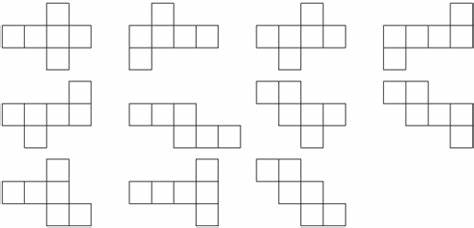
\includegraphics[width=12cm]{nets.jpg}
\caption{The 11 essentially different cube nets.}
\end{figure}

In this problem, we consider a generalization of the cube net, called \textit{cube hypernet}. For each face of a cube, we divide it into $k \times k$ small square cells. If we cut some edges of these small cells, the surface of the cube can be unfolded into 2-dimensional space, then the resulting flat shape is a cube hypernet. Clearly, cube nets are just a special type of cube hypernets where $k = 1$. The following picture illustrates a cube hypernet and explains how it is formed.

\begin{figure}[htb]
\centering

\tikzset{every picture/.style={line width=0.75pt}} %set default line width to 0.75pt        

\begin{tikzpicture}[x=0.75pt,y=0.75pt,yscale=-1,xscale=1]
%uncomment if require: \path (0,300); %set diagram left start at 0, and has height of 300

%Shape: Cube [id:dp5713421173433544] 
\draw   (92,119.87) -- (124.2,87.67) -- (199.43,87.67) -- (199.43,162.8) -- (167.23,195) -- (92,195) -- cycle ; \draw   (199.43,87.67) -- (167.23,119.87) -- (92,119.87) ; \draw   (167.23,119.87) -- (167.23,195) ;
%Straight Lines [id:da42563945957545957] 
\draw [color={rgb, 255:red, 208; green, 2; blue, 27 }  ,draw opacity=1 ][line width=3]    (92,119.87) -- (92,195) ;


%Straight Lines [id:da11360839227996866] 
\draw [color={rgb, 255:red, 208; green, 2; blue, 27 }  ,draw opacity=1 ][line width=3]    (92,119.87) -- (167.23,119.87) ;


%Straight Lines [id:da5837990090607357] 
\draw [color={rgb, 255:red, 208; green, 2; blue, 27 }  ,draw opacity=1 ][line width=3]  [dash pattern={on 7.88pt off 4.5pt}]  (124.2,87.67) -- (124.22,163.49) ;


%Straight Lines [id:da3949397955529803] 
\draw [color={rgb, 255:red, 208; green, 2; blue, 27 }  ,draw opacity=1 ][line width=3]    (125.08,86.84) -- (199.43,87.67) ;


%Straight Lines [id:da4851398910346689] 
\draw [color={rgb, 255:red, 208; green, 2; blue, 27 }  ,draw opacity=1 ][line width=3]    (167.23,119.87) -- (167.23,195) ;


%Straight Lines [id:da7311203923035952] 
\draw [color={rgb, 255:red, 208; green, 2; blue, 27 }  ,draw opacity=1 ][line width=3]    (199.43,87.67) -- (198.57,164.32) ;


%Straight Lines [id:da7022479459425415] 
\draw  [dash pattern={on 4.5pt off 4.5pt}]  (124.22,163.49) -- (199.43,162.8) ;


%Straight Lines [id:da7189806870957662] 
\draw  [dash pattern={on 4.5pt off 4.5pt}]  (124.22,163.49) -- (92,195) ;


%Straight Lines [id:da9178045604326999] 
\draw [color={rgb, 255:red, 0; green, 0; blue, 0 }  ,draw opacity=1 ] [dash pattern={on 0.84pt off 2.51pt}]  (145.93,104.17) -- (182.43,104.67) ;


%Straight Lines [id:da04301172838480838] 
\draw [color={rgb, 255:red, 0; green, 0; blue, 0 }  ,draw opacity=1 ] [dash pattern={on 0.84pt off 2.51pt}]  (92,157.43) -- (167.23,157.43) ;


%Straight Lines [id:da9145997008953277] 
\draw [color={rgb, 255:red, 0; green, 0; blue, 0 }  ,draw opacity=1 ] [dash pattern={on 0.84pt off 2.51pt}]  (129.61,120.12) -- (129.61,194.75) ;


%Straight Lines [id:da9400584505703131] 
\draw  [dash pattern={on 0.84pt off 2.51pt}]  (109.43,103.67) -- (109.43,176.67) ;


%Straight Lines [id:da4339187022384017] 
\draw  [dash pattern={on 0.84pt off 2.51pt}]  (92,157.43) -- (123.43,126.01) ;


%Straight Lines [id:da12326295357742123] 
\draw  [dash pattern={on 0.84pt off 2.51pt}]  (109.43,176.67) -- (183.43,176.67) ;


%Straight Lines [id:da859413357855844] 
\draw  [dash pattern={on 0.84pt off 2.51pt}]  (129.61,194.75) -- (161.82,163.15) ;


%Straight Lines [id:da22416829329673393] 
\draw  [dash pattern={on 0.84pt off 2.51pt}]  (162.25,87.25) -- (161.82,163.15) ;


%Straight Lines [id:da5602089262552088] 
\draw  [dash pattern={on 0.84pt off 2.51pt}]  (124.21,125.58) -- (199,125.99) ;


%Straight Lines [id:da9523299030375125] 
\draw  [dash pattern={on 0.84pt off 2.51pt}]  (167.23,157.43) -- (199,125.99) ;


%Straight Lines [id:da5451371565037118] 
\draw  [dash pattern={on 0.84pt off 2.51pt}]  (182.43,104.67) -- (183.43,176.67) ;


%Shape: Square [id:dp7591135470696151] 
\draw   (390,65) -- (414.33,65) -- (414.33,89.33) -- (390,89.33) -- cycle ;
%Shape: Square [id:dp917157522376586] 
\draw   (390,89.33) -- (414.33,89.33) -- (414.33,113.67) -- (390,113.67) -- cycle ;
%Shape: Square [id:dp6066190461876488] 
\draw   (414.33,65) -- (438.67,65) -- (438.67,89.33) -- (414.33,89.33) -- cycle ;
%Shape: Square [id:dp23412140295087092] 
\draw   (414.33,89.33) -- (438.67,89.33) -- (438.67,113.67) -- (414.33,113.67) -- cycle ;
%Shape: Square [id:dp39521998722950746] 
\draw   (390,113.67) -- (414.33,113.67) -- (414.33,138) -- (390,138) -- cycle ;
%Shape: Square [id:dp7597028280692992] 
\draw   (390,138) -- (414.33,138) -- (414.33,162.33) -- (390,162.33) -- cycle ;
%Shape: Square [id:dp9032016100512299] 
\draw   (414.33,113.67) -- (438.67,113.67) -- (438.67,138) -- (414.33,138) -- cycle ;
%Shape: Square [id:dp9862136660298677] 
\draw   (414.33,138) -- (438.67,138) -- (438.67,162.33) -- (414.33,162.33) -- cycle ;
%Shape: Square [id:dp2105696458351256] 
\draw   (390,162.33) -- (414.33,162.33) -- (414.33,186.67) -- (390,186.67) -- cycle ;
%Shape: Square [id:dp38203525928531445] 
\draw   (414.33,162.33) -- (438.67,162.33) -- (438.67,186.67) -- (414.33,186.67) -- cycle ;
%Shape: Square [id:dp07452681855437948] 
\draw   (390,186.67) -- (414.33,186.67) -- (414.33,211) -- (390,211) -- cycle ;
%Shape: Square [id:dp46685422276231514] 
\draw   (414.33,186.67) -- (438.67,186.67) -- (438.67,211) -- (414.33,211) -- cycle ;
%Shape: Square [id:dp1815129932944446] 
\draw   (438.67,113.67) -- (463,113.67) -- (463,138) -- (438.67,138) -- cycle ;
%Shape: Square [id:dp8928307047272608] 
\draw   (438.67,138) -- (463,138) -- (463,162.33) -- (438.67,162.33) -- cycle ;
%Shape: Square [id:dp3917633232801916] 
\draw   (463,113.67) -- (487.34,113.67) -- (487.34,138) -- (463,138) -- cycle ;
%Shape: Square [id:dp4091908537319717] 
\draw   (463,138) -- (487.34,138) -- (487.34,162.33) -- (463,162.33) -- cycle ;
%Shape: Square [id:dp3525235222171257] 
\draw   (365.67,113.67) -- (390,113.67) -- (390,138) -- (365.67,138) -- cycle ;
%Shape: Square [id:dp5339668640142305] 
\draw   (365.67,138) -- (390,138) -- (390,162.33) -- (365.67,162.33) -- cycle ;
%Shape: Square [id:dp8907339502163012] 
\draw   (341.33,113.67) -- (365.67,113.67) -- (365.67,138) -- (341.33,138) -- cycle ;
%Shape: Square [id:dp4554401476147847] 
\draw   (341.33,138) -- (365.67,138) -- (365.67,162.33) -- (341.33,162.33) -- cycle ;
%Shape: Square [id:dp633196329874429] 
\draw   (317,113.67) -- (341.33,113.67) -- (341.33,138) -- (317,138) -- cycle ;
%Shape: Square [id:dp062935463038297] 
\draw   (511.67,138) -- (536,138) -- (536,162.33) -- (511.67,162.33) -- cycle ;
%Shape: Square [id:dp8856843680936886] 
\draw   (487.34,113.67) -- (511.67,113.67) -- (511.67,138) -- (487.34,138) -- cycle ;
%Shape: Square [id:dp514905839618633] 
\draw   (487.34,138) -- (511.67,138) -- (511.67,162.33) -- (487.34,162.33) -- cycle ;
%Straight Lines [id:da9682499505773039] 
\draw [color={rgb, 255:red, 208; green, 2; blue, 27 }  ,draw opacity=1 ][line width=3]    (145.93,104.17) -- (162.25,87.25) ;


%Straight Lines [id:da17272908888168392] 
\draw [color={rgb, 255:red, 208; green, 2; blue, 27 }  ,draw opacity=1 ][line width=3.75]    (109.43,103.67) -- (145.93,104.17) ;


%Straight Lines [id:da7081830858409768] 
\draw [color={rgb, 255:red, 208; green, 2; blue, 27 }  ,draw opacity=1 ][line width=3.75]    (109.43,103.67) -- (92,119.87) ;


%Straight Lines [id:da379429243876815] 
\draw  [dash pattern={on 0.84pt off 2.51pt}]  (145.93,104.17) -- (129.61,120.12) ;


\end{tikzpicture}
\caption{A cube hypernet.}
\end{figure}

Identifying cube nets is a relatively easy job, however, this might not be true for cube hypernets. Here comes the challenge. Given a flat shape composed of small squares, determine whether it is a cube hypernet.

\subsection*{Input}

The first line of the input is a single integer $T$ $(1 \leq T \leq 30)$, denoting the number of test cases. 

For each test case, the first line contains two integers $h, w$ $(1 \leq h, w \leq 100)$, denoting the height and width of the input region. For the remaining $h$ lines, each containing $w$ characters, either \texttt{'\#'} or \texttt{'.'}. The character \texttt{'\#'} means that the square is part of the shape, while the character \texttt{'.'} means that the square is not part of the shape.

It is guaranteed that the input shape is nonempty and connected in four directions, and there is no hole inside the shape, not even a hole 8-connected to the outside. Also, the sum of $h \times w$ over all test cases does not exceed 35000.

\subsection*{Output}

For each test case, output \texttt{yes} in a line if the input shape is cube hypernet, and \texttt{no} otherwise.

\exmpv{cube}

\end{Problem}

\begin{Problem}{Acesrc and Girlfriend}{12}

Acesrc and his girlfriend are famous sweet lovers at Nanjing University second to none. They often wander along the streets near Xinjiekou, and taste takoyaki.

Xinjiekou is the central business district of Nanjing, consisting of $n$ crossroads and $m$ streets connecting some pairs of these crossroads. By every street there is a takoyaki bar, and Acesrc has a preference value for each of these bars. The streets are bidirectional.

Acesrc and his girlfriend choose a pair of crossroads as the starting point and the ending point; moreover, they choose a route between these two crossroads, and they walk along the streets in the route. Every crossroad appears in the route at most once. Once they encounter a takoyaki bar they will buy a serve of takoyaki from this bar. However, they can keep at most two serves of takoyaki. If, after buying a serve of takoyaki they have more than two serves, they will discard one serve with minimum preference value.

After reaching the ending point they begin to enjoy the takoyaki. Acesrc always eats the serve with lower preference value; however, if they only bought one serve, poor Acesrc will have nothing to eat. The clever Acesrc wants to know the minimum possible preference value of the serve he eats, given the starting point and the ending point of their route. Can you tell him the value?

\subsection*{Input}

The first line of input consists of a single integer $T$ $(1 \leq T \leq 100)$, the number of test cases. 

For each test case, the first line consists of three integers $n, m, q$ $(1 \leq n, q \leq 10^5, 1 \leq m \leq 2 \times 10^5)$, denoting the number of crossroads, streets in Xinjiekou, and the number of queries, respectively. Each of the next $m$ lines contains three integers $x, y, w$ $(1 \leq x, y \leq n, x \neq y, 1 \leq w \leq 10^9)$, denoting a street connecting the $x$th and the $y$th crossroads, with a takoyaki bar of preference value $w$ near the street. It is possible that multiple streets connect the same pair of crossroads. Each of the last $q$ lines are two integers $u, v$ $(1 \leq u, v \leq n, u \neq v)$, specifying a query that the starting point and ending point are the $u$th and the $v$th crossroads, respectively.

It is guaranteed that the sum of $n$ and the sum of $q$ over all test cases do not exceed $2.5 \times 10^5$, and the sum of $m$ does not exceed $5 \times 10^5$.

\subsection*{Output}

For each query of each test case, print the answer in one line. If Acesrc might have nothing to eat, print 0; if there is no path between the given starting and ending point, print -1.

\exmpv{girl}

\end{Problem}

\begin{Problem}{Acesrc and Good Numbers}{1}

Acesrc is a famous mathematician at Nanjing University second to none. Playing with interesting numbers is his favorite. Today, he finds a manuscript when cleaning his room, which reads

\begin{quote}
... Let $f(d, n)$ denote the number of occurrences of digit $d$ in decimal representations of integers $1, 2, 3, \cdots, n$. The function has some fantastic properties ...

... Obviously, there exist some nonnegative integers $k$, such that $f(d, k) = k$, and I decide to call them $d$-good numbers ...

... I have found all $d$-good numbers not exceeding $10^{1000}$, but the paper is too small to write all these numbers ...
\end{quote}

Acesrc quickly recollects all $d$-good numbers he found, and he tells Zou a question about $d$-good numbers: what is the maximum $d$-good number no greater than $x$? However, Zou is not good at mathematics, so he wants you to help him solve this problem.

\subsection*{Input}

The first line of input consists of a single integer $q$ $(1 \leq q \leq 1500)$, denoting the number of test cases. Each test case is a single line with two integers $d$ $(1 \leq d \leq 9)$ and $x$ $(0 \leq x \leq 10^{18})$.

\subsection*{Output}

For each test case, print the answer as a single integer in one line. Note that $0$ is trivially a $d$-good number for arbitrary $d$.

\exmpv{number}

\end{Problem}

\begin{Problem}{Acesrc and Hunting}{2}

Acesrc is a famous hunter at Nanjing University second to none. Recently, he set $n \times m$ traps in Yangshan Park, a park near Nanjing University Xianlin Campus, arranged in $n$ rows and $m$ columns. The rows are numbered $1$ through $n$ from bottom to up, and the columns are numbered $1$ through $m$ from left to right. The distance between two adjacent traps, both horizontally and vertically, is 1 meter.

Today, Acesrc happily finds that every trap he set has captured an animal. He decides to collect these hunted animals to make roast meat for his friends. However, collecting these animals normally is too boring, so he decides to find a route following the rules below:
\begin{itemize}
\item Acesrc can choose any trap to start; every time he collects the animal in the trap, and moves to some unvisited trap until all animals captured are collected;
\item The Euclidean distance he moves from one trap to the next trap should be between 1 meter and 3 meters exclusive; that is, the distance should be strictly greater than 1 meter and strictly less than 3 meters.
\end{itemize}

Acesrc has quickly collected all animals. Roo wonders how Acesrc collected these animals, but Acesrc buttons up his lip. Can you give a possible route to collect all the animals?

\subsection*{Input}

The first line of input consists of a single integer $T$ $(1 \leq T \leq 240)$, the number of test cases. Each test case is a single line of two integers $n, m$ $(1 \leq n, m \leq 100)$, denoting the size of the trap matrix.

\subsection*{Output}

For each test case, if it is impossible to find any valid route, print \texttt{NO} in a single line; otherwise, print \texttt{YES} in one line, followed by $n \times m$ lines describing the route, each of these lines containing two integers $x, y$ $(1 \leq x \leq n, 1 \leq y \leq m)$, denoting the position of a trap visited. If multiple solutions exist, print any.

\exmpv{hunting}

\end{Problem}

\begin{Problem}{Acesrc and String Theory}{7}

Acesrc is a famous string theorist at Nanjing University second to none. He insists on the principle that we should say an important thing $k$ times. He believes that every string that can be obtained by concatenating $k$ copies of some nonempty string is splendid. So, he always teaches newcomers, ``String theory problems are important! String theory problems are important! ... String theory problems are important!"

Today, he wants to examine whether the newcomers remember his instruction. He presents a string consisting of lower case letters and asks them the number of splendid substrings of the presented string. No one can solve this problem, and they will be scolded for hours. Can you help them solve this problem?

Note that equal splendid substrings occurred in different positions should be counted multiple times.

\subsection*{Input}

The first line of input consists of a single integer $T$ $(1 \leq T \leq 10)$, denoting the number of test cases. Each test case starts with a single line of an integer $k$ $(1 \leq k \leq 20)$. The second line of a test case is a string $S$ consisting of lower case letters only, the length of which is between $1$ and $3 \times 10^5$ inclusive. The sum of the lengths of all strings does not exceed $10^6$.

\subsection*{Output}

For each test case, print the answer as a single integer in a single line.

\exmpv{string}

\end{Problem}

\begin{Problem}{Acesrc and Travel}{2}

Acesrc is a famous tourist at Nanjing University second to none. During this summer holiday, he, along with Zhang and Liu, is going to travel to Hong Kong. There are $n$ spots in Hong Kong, and $n - 1$ bidirectional sightseeing bus routes connecting these spots. They decide to visit some spots by taking the buses.

However, Zhang and Liu have different preferences for these spots. They respectively set a satisfactory value for each spot. If they visit the $i$th spot, Zhang will obtain satisfactory value $a_i$, and Liu will obtain $b_i$. Starting with Zhang, they alternately decide the next spot to visit for the sake of fairness. There must be a bus route between the current spot and the next spot to visit. Moreover, they would never like to visit a spot twice. If anyone can't find such a next spot to visit, they have no choice but to end this travel.

Zhang and Liu are both super smart competitive programmers. Either want to maximize the difference between his total satisfactory value and the other's. Now Acesrc wonders, if they both choose optimally, what is the difference of total satisfactory values of Zhang and Liu?

\subsection*{Input}

The first line of input consists of a single integer $T$ $(1 \leq T \leq 30)$, denoting the number of test cases.

For each test case, the first line contains a single integer $n$ $(1 \leq n \leq 10^5)$, denoting the number of spots. Each of the next two lines contains $n$ integers, $a_1, a_2, \cdots, a_n$ and $b_1, b_2, \cdots, b_n$ $(0 \leq a_i, b_i \leq 10^9)$, denoting the 
satisfactory value of Zhang and Liu for every spot, respectively. Each of the last $n - 1$ lines contains two integers $x, y$ $(1 \leq x, y \leq n, x \neq y)$, denoting a bus route between the $x$th spot and the $y$th spot. It is reachable from any spot to any other spot through these bus routes.

It is guaranteed that the sum of $n$ does not exceed $5.01 \times 10^5$.

\subsection*{Output}

For each test case, print a single integer in one line, the difference of total satisfactory values if they both choose optimally.

\exmpv{travel}

\end{Problem}

\begin{Problem}{Andy and Data Structure}{15}

Andy is a famous data structure expert at Nanjing University second to none. One day he throws a plain dry data structure problem to his friends, but none of them can solve. How about you?

Given a tree rooted at node 1. Each node has a weight which is 0 initially. Define the distance between two nodes as the number of edges in the unique simple path between the two nodes. You need to perform these two types of operations:
\begin{itemize}
\item Type 1: given $a, x, y, z$, add $z$ to the weights of all $a$'s descendants (including $a$ itself) whose distances to $a$ are $x$ modulo $y$;
\item Type 2: given $a$, return the weight associated with node $a$.
\end{itemize}

\subsection*{Input}

The first line of the input is a single integer $T$ $(1 \leq T \leq 3)$, the number of test cases.

Each test cases starts with two integers $n, m$ $(1 \leq n, m \leq 300000)$, denoting that there are $n$ nodes (numbered $1$ through $n$) in the tree and you need to perform $m$ operations. The next line contains $n-1$ integers, $f_1, f_2, \cdots, f_{n-1}$ $(1 \leq f_i \leq i)$, specifying the edges of the trees; the $i$th integer denotes the parent of node $i+1$. The next $m$ lines describe the operations. Each line is either \texttt{1 a x y z} $(1 \leq a \leq n, 1 \leq x \leq n, 0 \leq y < x, 0 \leq z \leq 500)$, denoting an operation of type 1, or \texttt{2 a} $(1 \leq a \leq n)$, denoting an operation of type 2.

\subsection*{Output}

For each operation of type 2 in each test case, print the answer in one line.

\exmpv{ds}

\end{Problem}

\begin{Problem}{Andy and Maze}{15}

Andy is a famous explorer at Nanjing University second to none. One day he was trapped in a maze. The maze consisted of several rooms, and there was a precious gem in each room. There were also some bidirectional roads connecting some pairs of these rooms. It took some time to travel along the road in either direction.

Andy was in a room, but he didn't know which room he was in. Suddenly, he heard a low voice, saying that, ``if you want to get out of the maze, you must collect $k$ gems." Andy wanted to know, what was the minimum possible time to get out of the maze, or it was impossible at all? Note that he couldn't visit the same room more than once.

\subsection*{Input}

The first line of input consists of a single integer $T$ $(1 \leq T \leq 30)$, denoting the number of test cases. Each test case starts with a line of three integers $n, m, k$ $(2 \leq n \leq 10^4, 1 \leq m \leq 10^4, 2 \leq k \leq 6)$, denoting the number of rooms and the number of roads in the maze, and the number of gems he needed collect, respectively. The next $m$ lines, each containing three intergers $u, v, t$ $(1 \leq u, v \leq n, u \neq v, 1 \leq t \leq 10^8)$, specifying a road connecting the $u$th and the $v$th rooms, which takes $t$ minutes to travel in either direction. No two roads connect the same pair of rooms.
There are at most 5 test cases with $\max\{n, m\} > 100$.

\subsection*{Output}

For each test case, print the minimum possible time in minute to get out of the maze in one line. If it was impossible to get out of the maze, print \texttt{impossible} instead.

\exmpv{maze}

\end{Problem}

\begin{Problem}{Calabash and Landlord}{1}

Calabash is the servant of a landlord. The landlord owns a piece of land, which can be regarded as an infinite 2D plane.

One day the landlord set up two orthogonal rectangular-shaped fences on his land. He asked Calabash a simple problem: how many nonempty connected components is my land divided into by these two fences, both finite and infinite? Calabash couldn't answer this simple question. Please help him! 

Recall that a connected component is a maximal set of points not occupied by the fences, and every two points in the set are reachable without crossing the fence.

\subsection*{Input}

The first line of input consists of a single integer $T$ $(1 \leq T \leq 10000)$, the number of test cases. 

Each test case contains two lines, specifying the two rectangles. Each line contains four integers $x_1, y_1, x_2, y_2$ $(0 \leq x_1, y_1, x_2, y_2 \leq 10^9, x_1 < x_2, y_1 < y_2)$, where $(x_1, y_1), (x_2, y_2)$ are the Cartesian coordinates of two opposite vertices of the rectangular fence. The edges of the rectangles are parallel to the coordinate axes. The edges of the two rectangles may intersect, overlap, or even coincide.

\subsection*{Output}

For each test case, print the answer as an integer in one line.

\exmpv{landlord}

\end{Problem}

\begin{Problem}{Quailty and CCPC}{2}

Considering the overall difficulty of other problems, we invite Quailty to propose an easy problem for this contest.

Quailty accidentally won both gold medal and silver medal in 2017 CCPC final. The reason is explained as follows. According to the official rule, the number of gold medals was 10\% of the number of participating teams, rounded to the nearest integer. This is ambiguous when the fractional part of the result is exactly $0.5$. There were 115 participating teams, and the rank of Quailty's team was 12. The organizer originally decided to round down the number, so there were only 11 gold medals, and Quailty's team could only win the silver medal. Many people defended him against the organizer, saying that his team deserved the gold medal. Later, the organizer changed to round up the number, and Quailty's team finally won a gold medal.

Now, give you the scoreboard of a contest and the proportion of gold medal teams, could you determine whether there exists a team, such that they would win a gold medal were the number of gold medals rounded up when the fractional part is exactly $0.5$, and silver medal if rounded down?

A team ranks before another if they solved more problems or both teams solved an equal number of problems but they had less penalty time.

\textit{(Disclaimer: the background is fictitious and the problem is prepared by Nanjing University ICPC Training Team, not Quailty.)}

\subsection*{Input}

The first line of input consists of a single integer $T$ $(1 \leq T \leq 120)$, denoting the number of test cases.

Each test case starts with a line of two integers $n$ $(1 \leq n \leq 10^5)$, denoting the number of participating teams, and $d$ $(0 \leq d \leq 9)$, denoting that the proportion of gold medal teams is $10d\%$. For the next $n$ lines, each containing a string $s$ and two integers $p, t$ $(0 \leq p, t \leq 10^9)$, denoting the name of the team, the number of problems solved and the penalty time of the team, respectively. The name of the each team contains at least 1 and at most 10 latin letters. The names are case sensitive. No two teams have the same name. No two teams have the same penalty time. The sum of $n$ over all test cases does not exceed $10^6$.

\subsection*{Output}

For each test case, print the team name if there exists such team, or print \texttt{Quailty is very great} otherwise. It can be proved that there is at most one such team.

\exmpv{ccpc}

\end{Problem}

\begin{Problem}{Roundgod and Milk Tea}{5}

Roundgod is a famous milk tea lover at Nanjing University second to none. This year, he plans to conduct a milk tea festival. There will be $n$ classes participating in this festival, where the $i$th class has $a_i$ students and will make $b_i$ cups of milk tea.

Roundgod wants more students to savor milk tea, so he stipulates that every student can taste at most one cup of milk tea. Moreover, a student can't drink a cup of milk tea made by his class. The problem is, what is the maximum number of students who can drink milk tea?

\subsection*{Input}

The first line of input consists of a single integer $T$ $(1 \leq T \leq 25)$, denoting the number of test cases.

Each test case starts with a line of a single integer $n$ $(1 \leq n \leq 10^6)$, the number of classes. For the next $n$ lines, each containing two integers $a, b$ $(0 \leq a, b \leq 10^9)$, denoting the number of students of the class and the number of cups of milk tea made by this class, respectively.

It is guaranteed that the sum of $n$ over all test cases does not exceed $6 \times 10^6$.

\subsection*{Output}

For each test case, print the answer as a single integer in one line.

\exmpv{milk}

\end{Problem}

\end{document}
